On the front page of its website~\cite{reservio}, Reservio describes itself as a \enquote{free online scheduling software for gyms, fitness centers, hair studios, barbershops, nail salons, car repair, medical services, teachers and educational institutions, group events, and more.}

When a user first signs up for a business account, they are asked to provide the following information:
\begin{itemize}
    \item the name of their business;
    % https://www.grammarly.com/blog/comma-between-correlative-conjunction-sets/
    \item the type of their business, which can be either \enquote{Single appointments} (described as \enquote{the client books a service or an appointment at a specific time}) or \enquote{Group events} (described as \enquote{host multiple clients at the same event, lecture or course}); to change this business type later on, one must contact customer support;
    \item opening hours, which \enquote{determine the exact range of when your clients can make bookings} and can also be customized per employee;
    \item the physical address of their business;
    \item optionally the contact phone number of their business;
    \item and optionally other information about their business -- a website, a slogan, a description, and additional information about the physical address.
\end{itemize}

Users are also asked to add the services they would like to provide to their clients. Each service must have a name and a duration, and can optionally have a description, a price, a color (to visually differentiate it from other provided services), and an additional question to ask the customers (which can also serve as an input for a voucher code).

Lastly, users can also add staff members of the business who provide the previously added services, each with a name, a checklist of the services they provide, and optionally a short biography.

After the user completes the sign-up process, customers can access a booking website that is created for the business on a Reservio subdomain. When a customer accesses the booking website, they immediately see all the information about the business that was provided during the sign up. They then select a service for booking, a staff member (or \enquote{anyone available}), a date from a calendar picker, and a free time slot for the selected date. The customer can complete their booking either as a guest or by creating a Reservio account (or logging into an existing account). If the customer chooses to create an account, they can also see their booking history and cancel their bookings (in the settings, a business can set how long before the event can the bookings be canceled). The business user can also restrict in the settings who can create bookings to for example only existing clients or only clients with an account. As the last step of the booking process, the customer can answer the additional question that was added by the business, and they may also add a note. Afterwards, the customer is sent an email with the details of their booking.

For group events, the process is very similar, with the business user additionally specifying the capacity of an event. The customers can then book multiple spots for an event, as long as there is sufficient space available. Group events can also be marked as private by the business user, in which case they are not visible to the public and can only be accessed through a direct link.

The booking page iframe or simple booking components can also be embedded into another website. The booking website can be set as indexable by search engines and can use a custom domain instead of the Reservio subdomain (for premium accounts only). The layout and theme of the booking website can be somewhat customized as well, though most of the customizations are limited to premium accounts. There is an extensive API which can be used to integrate Reservio with other applications.

Business users can see their existing bookings in a calendar (also available as per staff member and per service views) which can be seen in the figure~\ref{fig:reservio}, as well as an overview of their clients. Premium users can have their calendar be synchronized with other popular calendar applications. Users can edit and cancel the existing bookings, as well as manually add new bookings and clients. Unreliable clients can be blocked and there is a CSV file import of clients as well. The amount of bookings a business can have is limited by different premium subscription plans.

Other available features include the ability to receive email and SMS notifications about new and canceled bookings (though SMS is limited to premium accounts), client reminders a set number of days or hours before a booked event, the option to limit the time of user data retention, and adding analytics to the booking website (such as Google Analytics and Meta Pixel; limited to premium accounts). Businesses can opt in to have their profile listed in a service marketplace (which customers can access through a separate application). One business account may be used by more staff members with separate login credentials and role-based permissions.

The platform also features online payments (which can be set as mandatory or optional), for which it takes a commission: This feature includes the handling of refunds when a customer cancels their booking and the possibility of long term memberships. However, according to Reservio~\cite{reservio}, this feature is currently only available in the Czech Republic where the company originates and for security reasons it does not work when a custom domain is set up for the booking website.

\begin{figure}
    \centering
    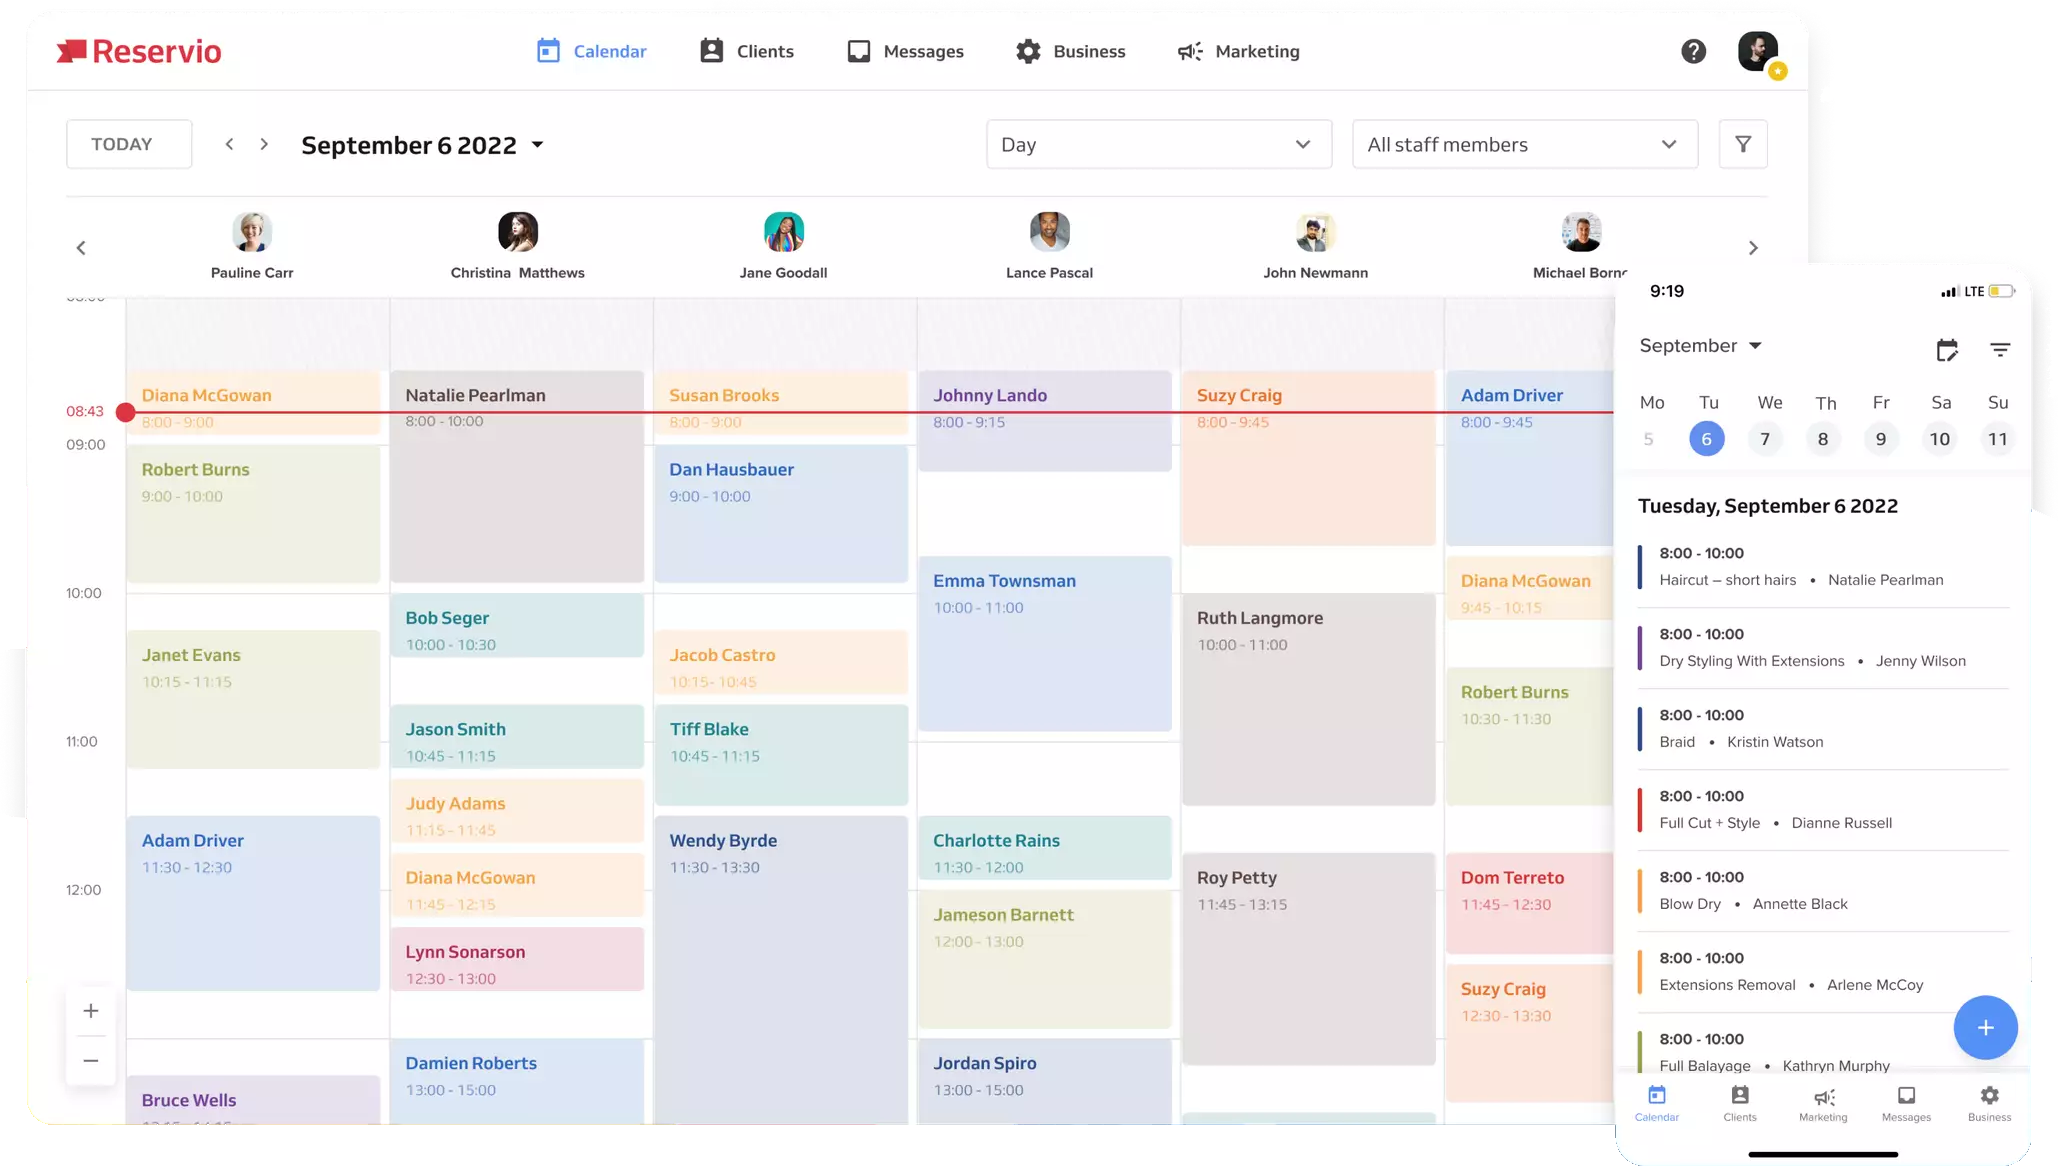
\includegraphics[width=1.0\textwidth]{content/existing_reservation_systems/reservio.png}
    \caption[Reservio]{Reservio~\cite{reservio}}
    \label{fig:reservio}
\end{figure}
